\documentclass[t]{sdqbeamer}
%\documentclass[c]{sdqbeamer}

\usepackage{listings}
\usepackage{graphicx}
\usepackage{tabularx}
\usepackage{multirow}
\usepackage{multicol}
\usepackage{tabulary}
\usepackage{colortbl}
\usepackage{tikzsymbols}
\usepackage{tikz}
\usetikzlibrary{positioning,fit,shapes}
\usepackage[lined,linesnumbered,ruled,noend]{algorithm2e}
\usepackage{bm}

\hypersetup{
	colorlinks=true,
	urlcolor=kit-orange
}

% set sdqbeamer options
\titleimage{blender-render}
\groupname{} % rendered at the bottom center of each slide
\grouplogo{ae+satres}
\selectlanguage{english}

% define title etc.pp.
\title{Practical SAT Solving}
\subtitle{Lecture 9 \unimp{\normalfont -- Redundancy Notions and Proofs of Unsatisfiability}}
\author{\underline{Ashlin Iser}, Dominik Schreiber}
\date{June 22, 2026}

% define commands
\input{l00-commands.tex}


\begin{document}

\begin{frame}[title white horizontal, picture=logos/blender-render, kitlogo=rgb]
	\titlepage
\end{frame}


\begin{frame}{Conflict-driven Clause Learning (CDCL)}
\vspace*{-1em}
\begin{columns}[T]
\begin{column}{.4\linewidth}
~\\[1em]
Recap: \highlow{Preprocessing}\\[1ex]
\begin{itemize}\itemsep1ex
    \item Subsumption
    \item Self-subsuming Resolution
    \item Bounded Variable Elimination
    \item Blocked Clause Elimination
    \item Relationship with Tseitin Encoding
    \item Scheduling\\[1ex]
    \begin{itemize}\itemsep1ex
        \item Heuristic Bounds
        \item Interleaving of Techniques (f.ex. Round Robin)
        \item \highlow{Inprocessing}: Interleave with solving
    \end{itemize}
\end{itemize}
\end{column}
\begin{column}{.55\linewidth}
\begin{algorithm}[H]
    \DontPrintSemicolon
    \caption{CDCL(CNF Formula $F$, \&Assignment A $\leftarrow \emptyset$)}
    
    \SetKwFunction{preprocessing}{\highlow{PREPROCESSING}}
    \SetKwFunction{inprocessing}{\highlow{INPROCESSING}}
    \SetKwFunction{propagation}{UNIT PROPAGATION}
    \SetKwFunction{branching}{BRANCHING}
    \SetKwFunction{conflictanalysis}{CONFLICT-ANALYSIS}
    \SetKwFunction{restart}{RESTART}
    \SetKwFunction{cleanup}{CLEANUP}

    \SetKwData{UNSAT}{UNSAT}
    \SetKwData{SAT}{SAT}
    
    \lIf {not \preprocessing} {
        \Return \UNSAT
    }
    \BlankLine
    \While {A is not complete} {
        \propagation\;
        \If {A falsifies a clause in $F$} {
            \lIf {decision level is $0$} {
                \Return \UNSAT
            }
            \Else {
                (clause, level) $\leftarrow$ \conflictanalysis\;
                add clause to $F$ and backtrack to level\;
                \textbf{continue}\;
            }
        }
        \lIf {\restart} {
            backtrack to level $0$
        }
        \lIf {\cleanup} {
            forget some learned clauses
        }
        \lIf {not \inprocessing} {
            \Return \UNSAT
        }
        \branching\;
    }
    \Return \SAT\;
\end{algorithm}
\end{column}
\end{columns}
\end{frame}


\begin{frame}{Propagation-based Redundancy Notions}
Let a formula $F$, and a literal $x$ be given.\\[1ex]
\begin{block}{Failed Literal Probing}
If $F \land x \vdash_{\mathop{UP}} \bot$, then $F \models \lnot x$\\[1ex]
$\implies$ add $\{ \lnot x \}$ to $F$
\end{block}~\\
\only<1>{\highlow{Recap: Meaning of $\vdash$ and $\models$?}}
\pause
\begin{example}[Failed Literal Probing]
Let $F := \bigl\{ \{a, b\}, \{a, \lnot b\} \bigr\}$.\\[1ex]
Probing with $\lnot a$ results in a conflict, i.e., $F \land \lnot a \vdash_{\mathop{UP}} \bot$.\\[1ex]
Ergo, we can deduce $F \equiv F \land a$.
\end{example}
\end{frame}
    

\begin{frame}{Propagation-based Redundancy Notions}
Let a formula $F$, a clause $C \in F$, and a literal $x \in C$ be given.~\\[1ex]
\begin{block}{Asymmetric Literal Elimination (ALE)}
If $F \setminus C \land \overline{C \setminus \{ x \}} \vdash_{\mathop{UP}} \overline x$, then $F \models C \setminus \{ x \}$.\\[1ex]
$\implies$ strengthen $C$ to $C \setminus \{ x \}$
\end{block}~\\
\only<1>{\highlow{Proof?}}
\pause
%
\begin{example}[Asymmetric Literal Elimination (ALE)]
Let $F := \bigl\{ \{a, b\}, \{\lnot b, \lnot c\}, \{a, c, d\} \bigr\}$, $C := \{a, c, d\}$, and $x := c$.\\[1ex]
ALE results in the following propagation: $\bigl\{ \{a, b\}, \{\lnot b, \lnot c\}, \{\lnot a \}, \{\lnot d\} \bigr\} \vdash_{\mathop{UP}} \lnot c$.\\[1ex]
Ergo, we can deduce $F \models \{a, d\}$.
\end{example}~\\
$F$ can not have a model which satisfies $\{a, c, d\}$, but not $\{a, d\}$.
\end{frame}
    

\begin{frame}{Propagation-based Redundancy Notions}
Let a formula $F$, a clause $C \in F$, and a literal $x \in C$ be given.\\[1ex]
\begin{block}{Asymmetric Tautology Elimination (ATE)}
If $F \setminus C \land \overline C \vdash_{\mathop{UP}} \bot$, then $F \models C$.\\[1ex]
$\implies$ remove $C$ from $F$
\end{block}~\\
\only<1>{\highlow{Does that remind you of something?}}
\pause
%
\begin{example}[Asymmetric Tautology Elimination (ATE)]
Let $F := \bigl\{ \{a, b, c\}, \{\lnot b, d\}, \{a, c, d\} \bigr\}$, and $C := \{a, c, d\}$.\\[1ex]
ATE results in the following propagation: $\bigl\{ \{a, b, c\}, \{\lnot b, d\}, \{\lnot a\}, \{\lnot c\}, \{\lnot d\} \bigr\} \vdash_{\mathop{UP}} \bot$,\\[1ex]
Ergo, we can deduce $F \equiv F \setminus \{a,c,d\}$.
\end{example}~\\
$\{a,c,d\}$ follows from the other clauses in $F$.
\end{frame}


\begin{frame}{Propagation-based Redundancy Notions}
\begin{block}{Variants: Efficient Algorithms and Implementations}
\begin{itemize}\setlength{\itemsep}{1em}
    \item \textbf{Hidden Tautology Elimination (HTE) / Hidden Literal Elimination (HLE)}\\[3pt]
    Restricted forms of ATE/ALE which only propagate over binary clauses.\\[3pt]
    \item \textbf{Unhiding}: Efficient \textbf{HLE} algorithm based on randomized DFS and the parenthesis theorem%
    \footnote{\href{https://link.springer.com/chapter/10.1007/978-3-642-21581-0_17}{2011, Heule et al., Efficient CNF Simplification Based on Binary Implication Graphs}}\\[3pt]
    DFS assigns each node \emph{entry/exit timestamps}; transitivity in the BIG is read off in $O(1)$:
    \begin{itemize}\setlength{\itemsep}{2pt}
        \item \highlo{Hidden literal:} if timestamps show $\lnot a_1 \to a_2$\; (i.e.\ $a_1 \lor a_2$ is already implied), remove $a_2$ from the clause
        \item \highlo{Failed literal:} if $a \to \lnot a$ ($a$ is an ancestor of its own negation), then $a$ is globally false, no separate probing needed
    \end{itemize}
    % \item \textbf{Vivification}:
    % Interleave assignment and propagation to detect ATs / ALs early.\\[3pt]
    % \begin{itemize}\setlength{\itemsep}{2pt}
    %     \item Assign literals of $C$ one by one and propagate
    %     \item \highlo{Conflict} $\Rightarrow$ strengthen $C$ to the literals assigned so far
    %     \item \highlo{Literal propagated} $\Rightarrow$ remove it from $C$
    % \end{itemize}
    \item \textbf{Distillation}:
    Sort literals and clauses to simulate a trie, reusing propagations that share a common prefix.\\[3pt]
    $\Rightarrow$ Detect ATs / ALs for \emph{multiple clauses} at once.\\
\end{itemize}
\end{block}
\end{frame}


\begin{frame}{Vivification}
\vspace*{-1em}
Given clause $C = (a_1 \lor a_2 \lor \cdots \lor a_k)$. Sequentially assign $\lnot a_1, \lnot a_2, \ldots$ and propagate over $F \setminus \{C\}$.\\[1ex]
\begin{block}{What can happen after assigning $P := \{\lnot a_1, \ldots, \lnot a_{i \leq k}\}$ and propagating?}
\begin{itemize}\setlength{\itemsep}{1em}
    \item \highlo{Conflict $(\bot)$}: the negated prefix $\overline P$ is contradictory w.r.t.\ $F \setminus \{C\}$.
    \begin{itemize}\normalsize\setlength{\itemsep}{5pt}
        \item[] \only<1>{\highlow{What can we do in this case?}}\onslide<2->{$\Rightarrow$ \textbf{Clause elimination:} remove $C$.}
        \item[] \only<2>{\highlow{Why is that sound?}}\onslide<3->{$\overline P \subseteq \overline{C}$ gives $F \setminus C \land \overline{C} \vdash_{\mathit{UP}} \bot$, the ATE condition $\Rightarrow F \models C$.}
    \end{itemize}
    \item \highlo{for some $a \in C \setminus P, a$ is propagated true}: $\overline P \vdash_{\mathit{UP}} a$.
    \begin{itemize}\normalsize\setlength{\itemsep}{5pt}
        \item[] \only<4>{\highlow{What can we do in this case?}}\onslide<5->{$\Rightarrow$ \textbf{Clause truncation:} drop all unprocessed literals $C \setminus (P \cup \{a\})$.}
        \item[] \only<5>{\highlow{Why is that sound?}}\onslide<6->{$F \models \overline P \rightarrow a$, so $P \cup \{a\}$ already \emph{subsumes} $C$.}
    \end{itemize}
    \item \highlo{for some $a \in C \setminus P, a$ is propagated false}: $a$ can never help satisfy $C$ in this context.
    \begin{itemize}\normalsize\setlength{\itemsep}{5pt}
        \item[] \only<7>{\highlow{What can we do in this case?}}\onslide<8->{$\Rightarrow$ \textbf{Literal elimination:} remove $a$ and continue.}
        \item[] \only<8>{\highlow{Why is that sound?}}\onslide<9->{$\overline P \subseteq \overline{C \setminus \{a\}}$ gives $F \setminus C \land \overline{C \setminus \{a\}} \vdash_{\mathit{UP}} \lnot a$, the ALE condition $\Rightarrow F \models C \setminus \{a\}$.}
    \end{itemize}
\end{itemize}
\end{block}
\end{frame}


\begin{frame}{Recap.}
\begin{block}{Propagation-based Preprocessing}
    \begin{itemize}\setlength{\itemsep}{1em}
        \item Propagation-based Redundancy Notions:\\[1ex]
        Failed Literal Probing, Asymmetric Literal Elimination, Asymmetric Tautology Elimination
        \item Efficient Implementation of Propagation-based Redundancy Removal with Binary Implication Graphs (BIGs)
        \item Vivification and Distillation: Interleaving Propagation with Clause Strengthening and Elimination
    \end{itemize}
\end{block}
\begin{block}{Next Up}
    Proofs of Unsatisfiability
\end{block}
\end{frame}

\begin{frame}{Relationship with Proof Checking}
\begin{block}{Generalizations of Blocked Clauses}~\\
\begin{itemize}\setlength{\itemsep}{1em}
    \item \textbf{Reverse Unit Propagation (RUP)}\\[1pt]
    A clause has the property RUP if and only if it is an Asymmetric Tautology (AT).\\[1ex]
    CDCL's learned clauses are RUP at the moment of their learning.
    \item \textbf{Resolution Asymetric Tautologies (RATs)}\\[1pt]
    A clause $C$ is a RAT in a formula $F$ if it contains a literal $x$ such that\\
    \highlo{each resolvent in $C \otimes_x F_{\overline x}$ is an asymmetric tautology}.\\[1ex]
    Blocked Sets in particular are RATs.
\end{itemize}
~\\
\end{block}
\end{frame}


\begin{frame}{Proof Checking}
\vspace*{-2em}
SAT Solvers are complex software systems, and bugs are not uncommon.
\begin{block}{Trustworthiness of SAT Solvers}
\begin{itemize}\setlength{\itemsep}{1ex}
    \item For satisfiable instances, SAT solvers can output the found assignment
    \item For unsatisfiable instances, SAT solvers can output a proof of unsatisfiability
    \item Both can be checked independently from the solver by much simpler, and \textbf{formally verified program}.
\end{itemize}
\end{block}
\begin{example}[Applications of Proof Checking]
Unsatisfiability of a formula might proof important properties of the problem at hand, such as:\\
\begin{itemize}
    \item Absence of certain bugs in a hardware design or software verification, 
    \item Optimality of a certain makespan in planning
    \item etc. pp.
\end{itemize} 
\end{example}
\begin{block}{Feasibility of Proof Checking}
    RAT proof checking is polynomial in the proof-size, but proof-size is worst-case exponential in the formula-size.\\[1ex]
    \textbf{Pragmatics:}  if we could generate it, we can also check it.
\end{block}
\end{frame}


\begin{frame}{Proof Systems: Motivating Example}
\begin{example}[Mutilated Chessboards]
Let a chessboard be given with two diagonally opposite corners removed.\\
Is it possible to cover the remaining board with dominoes?\\[1ex]
\visible<2>{\textbf{Human:} No, because each dominoe covers exactly one black and one white field, and there are two more black fields than white fields.}
\begin{center}

\includegraphics[width=.2\linewidth]{figures/l07/mcb0.png}
\end{center}
\end{example}
\end{frame}


\begin{frame}{Proof Systems: Motivating Example}
\begin{example}[Mutilated Chessboards]
Let a chessboard be given with two diagonally opposite corners removed.\\
Is it possible to cover the remaining board with dominoes?\\[1ex]
\textbf{SAT Solver:} Let's try and learn.\\
\begin{tabularx}{\linewidth}{XXX}
    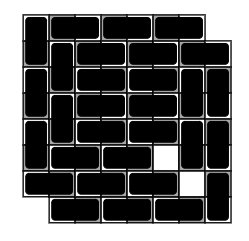
\includegraphics[width=.8\linewidth]{figures/l07/mcb1.png} &
    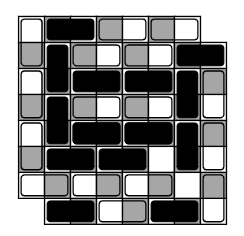
\includegraphics[width=.8\linewidth]{figures/l07/mcb2.png} &
    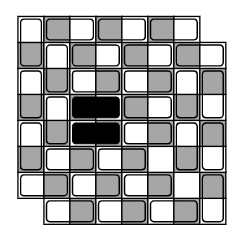
\includegraphics[width=.8\linewidth]{figures/l07/mcb3.png}\\
    \hline
    Impasse Detected & $\rightarrow$ Resolution & $\rightarrow$ More powerful Proof-system%
    \footnote{Example taken from SAT lecture of \href{https://www.cs.cmu.edu/~mheule/}{Marijn J.H. Heule}}
\end{tabularx}
\end{example}
\end{frame}


\begin{frame}{Proof Complexity}
Proof complexity is the study of the size of proofs in different proof systems.\\[1ex]
\begin{block}{Relationship with SAT Solving}
\begin{itemize}\setlength{\itemsep}{1ex}
\item Static analysis without algorithmic considerations
\item Questions of automizability not addressed
\item Lower bounds on proof size tell us how good a SAT solver can be in the best case 
\item Upper bounds on proof size tell us how good a SAT solver should be
\end{itemize}
\end{block}
~\\
\textbf{In the following:} three proof systems of \highlo{increasing power or generality}.
\begin{center}\small
\highlo{1.~Resolution} $\;\rightarrow\;$ \highlo{2.~Extended Resolution} $\;\rightarrow\;$ \highlo{3.~Blocked Clauses}
\end{center}
\end{frame}


\begin{frame}{Proof Systems \unimp{\normalfont -- 1. Resolution}}
\begin{center}\small
\highlo{1.~Resolution} $\;\rightarrow\;$ \unimp{2.~Extended Resolution} $\;\rightarrow\;$ \unimp{3.~Blocked Clauses}
\end{center}
\begin{block}{Resolution}
\begin{itemize}\setlength{\itemsep}{1ex}
    \item Preserves equivalence
    \item CDCL is as powerful as General Resolution
    \item Well-known Exponential Lower Bounds:\\[1ex]
    For example, proofs of unsatisfiability of Pigeon Hole formulas\\ 
    are necessarily of exponential length in the resolution proof system (Haken 1985)
    \item Heuristic for Finding Resolution Proofs: CDCL
\end{itemize}
\end{block}
\end{frame}


\begin{frame}{Proof Systems \unimp{\normalfont -- 2. Extended Resolution}}
\begin{center}\small
\unimp{1.~Resolution} $\;\rightarrow\;$ \highlo{2.~Extended Resolution} $\;\rightarrow\;$ \unimp{3.~Blocked Clauses}
\end{center}
\begin{block}{Extended Resolution (Tseitin 1966)}
\begin{itemize}\setlength{\itemsep}{1ex}
    \item Preserves satisfiability
    \item Extension rule:\\
    incorporate $x \leftrightarrow a \land b$ for some $a,b$ in the formula and a new variable $x$
    \item Strictly more powerful than Resolution
    \item No Lower Bounds known
    \item (Cook 1967) polynomial sized ER proof for PH formulas\\[1ex]
    $\Rightarrow$ exponentially shorter than any resolution proof
\end{itemize}
\end{block}
\end{frame}


\begin{frame}{Proof Systems \unimp{\normalfont -- 3. Blocked Clauses}}
\begin{center}\small
\unimp{1.~Resolution} $\;\rightarrow\;$ \unimp{2.~Extended Resolution} $\;\rightarrow\;$ \highlo{3.~Blocked Clauses}
\end{center}
\begin{block}{Blocked Clauses (Kullmann 1999)}
\begin{itemize}\setlength{\itemsep}{1ex}
    \item Preserves satisfiability
    \item Generalization of Extended Resolution
    \item Allows the addition and removal of blocked clauses\\[1ex]
    $\Rightarrow$ no need to introduce a defining equivalence explicitly
    \item No Lower Bounds known
\end{itemize}
\end{block}
\end{frame}


\begin{frame}{Stronger Proof Systems without New Variables}
\vspace*{-0.5em}
Extended Resolution and Blocked Clauses gain power by \highlo{introducing new variables}.\\[1ex]
\highlow{Can we obtain equally short proofs \emph{without} new variables?}
\begin{block}{Key relaxation: redundancy instead of implication}
A clause $C$ is \highlo{redundant} w.r.t.\ $F$ if $F$ and $F \land C$ are \emph{equisatisfiable}.\\[1ex]
$\Rightarrow$ $C$ need \textbf{not} be implied by $F$; it suffices that adding it preserves satisfiability.
\end{block}
\begin{example}[Redundant but \emph{not} implied]
$F := \bigl\{(a \lor b),\ (\lnot a \lor \lnot b)\bigr\}$ has exactly the models $\{\lnot a, b\}$ and $\{a, \lnot b\}$.\\[1ex]
Adding $C := (a)$ keeps $F$ satisfiable (model $\{a, \lnot b\}$), yet $F \not\models C$\\
since the model $\{\lnot a, b\}$ falsifies $C$.
\end{example}
\textbf{Background:} such systems can \highlo{polynomially simulate Extended Resolution}, e.g.\ short proofs of pigeon hole / mutilated chessboard without any new variables.
\end{frame}


\begin{frame}{Certifying Redundancy: the Witnessing Assignment}
How can we \emph{certify} that adding $C$ preserves satisfiability?\\[1ex]
\begin{block}{Redundancy via a witness}
Let $\alpha := \overline C$ be the assignment \highlo{blocked by $C$} (it falsifies every literal of $C$).\\[1ex]
$C$ is redundant w.r.t.\ $F$ $\quad\iff\quad$ there is a \highlo{witness} $\omega$ \quad with $\omega \models C \quad \text{and} \quad F|_\alpha \models F|_\omega.$\\[1ex]
{\small Notation: $F|_\beta$ removes from $F$ all clauses satisfied by $\beta$ and all literals falsified by $\beta$.}
\end{block}
\textbf{Intuition:} every model of $F$ that falsifies $C$ can be \highlo{repaired} into a model of $F \land C$ by patching it with $\omega$.
~\\[1em]
\begin{example}[Witness for $C=(a)$ in $F=\bigl\{(a\lor b),(\lnot a\lor \lnot b)\bigr\}$]
$\alpha = \{\lnot a\}$, \quad witness $\omega = \{a, \lnot b\}$ (which satisfies $C$).\\[1ex]
$F|_\alpha = \bigl\{(b)\bigr\}$ \quad and \quad $F|_\omega = \emptyset\;(\top)$, \quad so $F|_\alpha \models F|_\omega$ holds.
\end{example}
\end{frame}


\begin{frame}{Redundancy Theorem: Proof}
\vspace*{-2ex}
Let $F$ be a formula, $C$ a non-empty clause, and $\alpha = \overline C$ the assignment blocked by $C$.\\
$C$ is redundant with respect to $F$ \emph{if and only if} there exists an assignment $\omega$ such that $\omega$ satisfies $C$ and $F|_\alpha \models F|_\omega$.

\only<1>{
\begin{block}{\textbf{Proof ``only if''}}
\highl{Assume $F$ and $F \land C$ are equisatisfiable.} \highlo{Show that there exists an $\omega$ satisfying $C$ and $F|_\alpha \models F|_\omega$.}\\[1ex]
If $F|_\alpha$ is unsatisfiable, then the semantic implication trivially holds.\\[1ex]
Assume now that $F|_\alpha$ is satisfiable, implying that F is satisfiable.\\[1ex]
Since $F$ and $F \land C$ are equisatisfiable, there exists an assignment $\omega$ that satisfies both $F$ and $C$.\\[1ex]
Since $\omega$ satisfies F, it holds that $F|_\omega = \emptyset$ and so trivially $F|_\alpha \models F|_\omega$.
\end{block}
}

\only<2>{
\begin{block}{\textbf{Proof ``if''}}
\highl{Assume there exists an assignment $\omega$ satisfying $C$ and $F|_\alpha \models F|_\omega$.} \highlo{Show that $F$ and $F \land C$ are equisatisfiable.}\\[1ex]
Let $\gamma$ be a (total) assignment that satisfies $F$ and falsifies $C$.\\
Since \highlow{$\gamma$ satisfies $F$}, it must satisfy \highlow{$F|_\alpha$ and} since $F|_\alpha \models F|_\omega$, it must also satisfy \highlow{$F|_\omega$}.\\[1ex]
Now, we can turn $\gamma$ into a satisfying assignment $\gamma'$ for $F \land C$ as follows:\\
% As $\gamma$ falsifies $C$, it coincides with $\alpha$ on $\vars{C}$.\\
$$
\gamma'(x) = \begin{cases} 
    \omega(x) & \text{if } x \in \vars{\omega}\\ 
    \gamma(x) & \text{otherwise}
\end{cases}
$$
Since $\omega$ satisfies $C$, \highlow{$\gamma'$ satisfies $C$}.\\[1ex]
Since $\gamma$ satisfies $F|_\omega$ -- and $\vars{F|_\omega} \subseteq \vars{\gamma} \setminus \vars{\omega}$ -- so \highlow{$\gamma'$ satisfies $F$}.\\[1ex]
$\Rightarrow$ $\gamma'$ satisfies $F \land C$.
\end{block}
}
\end{frame}


\begin{frame}{In Practice: Propagation Redundancy (PR)}
\vspace*{-0.7em}
Deciding $F|_\alpha \models F|_\omega$ is coNP-hard: it asks whether \emph{every} assignment satisfying $F|_\alpha$ also satisfies $F|_\omega$, i.e.\ whether $F|_\alpha \land \lnot F|_\omega$ is \highlo{unsatisfiable}.
\begin{block}{Propagation Redundant (PR) clause}
$C$ is \highlo{PR} w.r.t.\ $F$ with witness $\omega$ if $\;\omega \models C\;$ and $\;F|_\alpha \vdash_{UP} F|_\omega$.
\end{block}
\highlo{Replace $\models$ by unit propagation $\vdash_{UP}$.} %A given \highlo{(clause, witness)} pair $(C, \omega)$ is verified in \highlo{polynomial time}: set $\alpha := \overline C$, check $\omega \models C$, and for \emph{each} $D \in F|_\omega$ assert $F|_\alpha \land \overline D \vdash_{UP} \bot$ (one linear UP run) $\Rightarrow$ overall polynomial.\\[1ex]
~\\[1ex]
% \textbf{Generalizing RAT:} RAT certifies a clause $C$ alone, using the \emph{implicit} witness ``$\alpha$ with the pivot $x \in C$ flipped''. PR carries the witness \highlo{explicitly}, so $\omega$ may flip \emph{several} variables, not just one of $C$.
% \begin{itemize}\setlength{\itemsep}{1pt}
%     \item Implicit RAT witness $\omega=\{a\}$: $F|_\omega=\{(\lnot b)\}$, $F|_\alpha=\{(b)\}\not\vdash_{UP}(\lnot b)$ -- \highlo{fails}.
%     \item Explicit witness $\omega=\{a,\lnot b\}$ flips $b$ too: $F|_\omega=\emptyset$ -- \highlo{succeeds}.
% \end{itemize}
\vfill
PR clauses need a witness $\omega$. But where do we \emph{find} one cheaply?\\
Up next: \highlo{autarkies}, a class of assignments that come \highlo{with their witness for free}.
\end{frame}


\begin{frame}{Autarkies}
\vspace*{-3.5ex}
\begin{block}{Autarky}
    Let a formula $F$ and a partial assignment $A$ be given. A clause $C \in F$ is \dots \\[1ex]
    \begin{itemize}\setlength{\itemsep}{0.5ex}
        \item \dots \highlo{touched} by $A$ if it contains a variable assigned in $A$
        \item \dots \highlo{satisfied} by $A$ if it contains a literal assigned to $\true$ by $A$
    \end{itemize}~\\[-1ex]
    An autarky is a partial assignment $A$ such that \highlo{all touched clauses are satisfied}.
\end{block}
%
Let $\alpha$ be an autarky of $F$. Then, $F$ and $F|_\alpha$ are equisatisfiable.
All clauses touched by an autarky can be removed.\\[1ex]
%
\textbf{Edge Cases:} Pure Literals and Satisfying Assignments are Autarkies\\
\textbf{Application in Inprocessing:} Kissat analyses assignments found by sprints of local search to find autarkies.\\[1ex]
%
\begin{exampleblock}{Example}
    The partial assignment $A = \{ \lnot a, \lnot c \}$ is an autarky for $F := \bigl\{\{ \lnot a, b \}, \{ b, \lnot c \}, \{ a, \lnot b, \lnot c \}\bigr\}$, with witness $\omega = A = \{ \lnot a, \lnot c \}$.
\end{exampleblock}
\end{frame}


\begin{frame}{Conditional Autarkies}
\vspace*{-2ex}
A plain autarky must satisfy \emph{all} touched clauses.\\
\highlo{Relax it conditionally:} require the autarky property only \emph{after} fixing some literals $\alpha_{con}$.\\[1ex]
\begin{block}{Conditional Autarkies}
An assignment $\alpha = \alpha_{con} \cup \alpha_{aut}$ is a conditional autarky of $F$ if $\alpha_{aut}$ is an autarky of $F|_{\alpha_{con}}$\\[1ex]
Then $F$ and $F \land (\alpha_{con} \rightarrow \alpha_{aut})$ are equisatisfiable.
\end{block}

\begin{example}[Pruning Branches with a Conditional Autarky]
Let $F := \bigl\{\{x, y\}, \{x, \lnot y\}, \{\lnot y, \lnot z\}\bigr\}$, and let $\alpha_{con} = \{x\}$ and $\alpha_{aut} = \{\lnot y\}$.\\[0.5ex]
Then $F|_{\alpha_{con}} = \bigl\{\{\lnot y, \lnot z\}\bigr\}$ and $\alpha_{aut} = \{\lnot y\}$ is an autarky of $F|_{\alpha_{con}}$, such that $\{x\} \cup \{\lnot y\}$ is a conditional autarky of $F$.\\[0.5ex]
We can thus learn the clause $\{\lnot x, \lnot y\}$, with witness $\omega = \{x, \lnot y\}$.
\end{example}
A conditional autarky \emph{is} the redundancy witness $\omega$ for the pruning clause. Next we \highlo{search} for it automatically while solving.
\end{frame}


\begin{frame}{Satisfaction Driven Clause Learning (SDCL)}
\textbf{Idea:} Also learn clauses if no conflict is detected, but a positive reduct is satisfiable.\\[1ex]

\begin{block}{Positive Reduct}
Let a formula $F$ and a partial, non-conflicting assignment $\alpha$ be given.\\[1ex]
The positive reduct $p(F, \alpha)$ is the formula that contains all clauses of $F$ satisfied by $\alpha$ and a clause $C := \lnot \alpha$.\\[1ex]
A satisfying assignment $\omega$ of the positive reduct $p(F,\alpha)$ is a conditional autarky of $F$, i.e.\ exactly the \highlo{redundancy witness $\omega$} for the pruning clause $\lnot \alpha$.\\[1ex]
$\Rightarrow$ if the positive reduct is satisfiable, then the branch $\alpha$ can be pruned.
\end{block}~\\
\textbf{Key Idea of SDCL:}\\[1ex]
While solving a formula, check the positive reducts of current assignments $\alpha$ for satisfiability.\\[1ex]
If $p(F, \alpha)$ is satisfiable, prune the branch $\alpha$.\\[1ex]
Positive reducts are typically very easy to solve.
\end{frame}


\begin{frame}{From Modern to ``Post-modern'' SAT Solving}
Problem: Automizability, how to find such short proofs?~\\[1ex]
\begin{block}{Solving the Problem of Automizability: Practical Approaches}
\begin{itemize}\setlength{\itemsep}{1em}
\item \textbf{Resolution}: Clause Learning\\[1ex]
$\bm\rightarrow$ \emph{any classic CDCL implementation}
\item \textbf{Extended Resolution}: Structural Boundend Variable Addiction (SBVA).\\[1ex]
$\bm\rightarrow$ \texttt{SBVA-CaDiCaL}: Winner of SAT Competition 2023
\item \textbf{PReLearning}: Preprocessing adds specific Propagation Redundant (PR) clauses\\[1ex]
$\bm\rightarrow$ \texttt{KissatMAB-Prop}: Winner of SAT Competition 2023 on UNSAT instances
\item \textbf{Symmetry Breaking Predicates}: Exclusion of Symmetric Solutions\\[1ex]
$\bm\rightarrow$ \texttt{BreakId-Kissat}: Special Price at SAT Competition 2023
\end{itemize}
\end{block}
\end{frame}


\begin{frame}{Recap.}
\begin{block}{Recap.}
\begin{itemize}\setlength{\itemsep}{1em}
    \item Propagation-based Redundancy Notions
    \item Proof Systems: Resolution, Extended Resolution, Blocked Clauses, Implication-based Redundancy
    \item Autarkies, Conditional Autarkies, and Satisfaction Driven Clause Learning (SDCL)
\end{itemize}
\end{block}
\end{frame}


\begin{frame}{References: Redundancy and Propagation Redundancy}
\begin{itemize}\setlength{\itemsep}{1.2em}
    \item \href{https://doi.org/10.1007/s10817-019-09516-0}{Heule, Kiesl, Biere (2019), \emph{Strong Extension-Free Proof Systems}}\\[2pt]
    Introduces \highlo{redundancy via a witness} and the redundancy theorem; defines the SPR/PR family of proof systems without new variables.
    \item \href{https://doi.org/10.1007/978-3-319-63046-5_9}{Heule, Kiesl, Biere (2017), \emph{Short Proofs Without New Variables}}\\[2pt]
    Defines \highlo{propagation-redundant (PR) clauses} and shows they admit short proofs (e.g.\ pigeon hole) without introducing new variables.
    \item \href{https://cakeml.org/tacas21.pdf}{Tan, Heule, Myreen (TACAS 21), \texttt{cake\_lpr}}\\[2pt]
    A \highlo{formally verified} PR proof checker, giving machine-checked trust in PR-based unsatisfiability proofs.
    \item \href{https://doi.org/10.1007/978-3-319-70389-3_12}{Heule et al.\ (2017), \emph{PRuning Through Satisfaction}}\\[2pt]
    Introduces \highlo{satisfaction-driven clause learning (SDCL)} via positive reducts and conditional autarkies.
    \item \href{https://doi.org/10.1016/0166-218X(85)90050-2}{Monien, Speckenmeyer (1985), \emph{Solving satisfiability in less than $2^n$ steps}}\\[2pt]
    Origin of \highlo{autark assignments}, the basis for autarky-based simplification.
\end{itemize}
\end{frame}

\end{document}
